
%======================================================================
% GÓI 1 (VIẾT LẠI): MỞ ĐẦU VÀ BẰNG CHỨNG VĨ MÔ VỀ "NGHỊCH LÝ PHÁT TRIỂN"
% (Phần 1: Tăng trưởng và Thành tựu)
%======================================================================

\chapter{越南外部质量保障体系现状分析}
\label{chap:thuc_trang}

\section*{引言}
\addcontentsline{toc}{section}{引言}

本章将对越南高等教育(GDĐH)外部质量保障(ĐBCL)体系的现状进行深入和多维度的分析,重点关注2015年至2024年这一强劲转型阶段。本章将运用第二章所论证的V-AQA理论模型视角,重点“解剖”一个深刻的\textbf{发展悖论(development paradox)}:即规模和投入指标的爆炸性增长,并未伴随着产出质量及与劳动力市场契合度的相应提升。

通过综合分析宏观统计数据、世界银行等权威国际组织的报告、学术研究,特别是通过图表进行可视化的数据,本章将提供坚实的科学论据。目标不仅是描述现状,更是要解释阻碍质量提升努力的系统性“瓶颈”和“恶性循环”。从而,本章将为后续章节提出战略性解决方案奠定坚实的实践基础。

\section{越南高等教育中的发展悖论}
\label{sec:nghich_ly_phat_trien_vimo}

2015-2024年阶段标志着越南高等教育一个充满变动的转型历程,揭示了一个深刻的发展悖论。一方面,该体系在教育大众化、扩大培养规模以及提升投入资源质量方面取得了前所未有的成就。另一方面,这些关于“量”的成就,却掩盖了关于“质”的持续挑战,体现在毕业生技能与劳动力市场实际需求之间日益扩大的不匹配。分析此悖论的两个方面,是理解该体系核心挑战的先决条件。

\subsection{悖论的第一面:规模的爆炸性增长与投入资源的改善}
\label{subsec:ve_thu_nhat_nghich_ly}

不可否认,越南高等教育在扩大民众教育机会方面取得了令人瞩目的进展。这一时期见证了强劲的大众化进程,体现在办学机构网络的拓展和学生规模的飞跃式增长。

\subsubsection{拓展教育网络与培养规模}

过去十年越南高等教育体系发展的全貌,通过图\ref{fig:so_truong_quy_mo_sv}得以清晰展现。

\begin{figure}[h!]
    \centering
    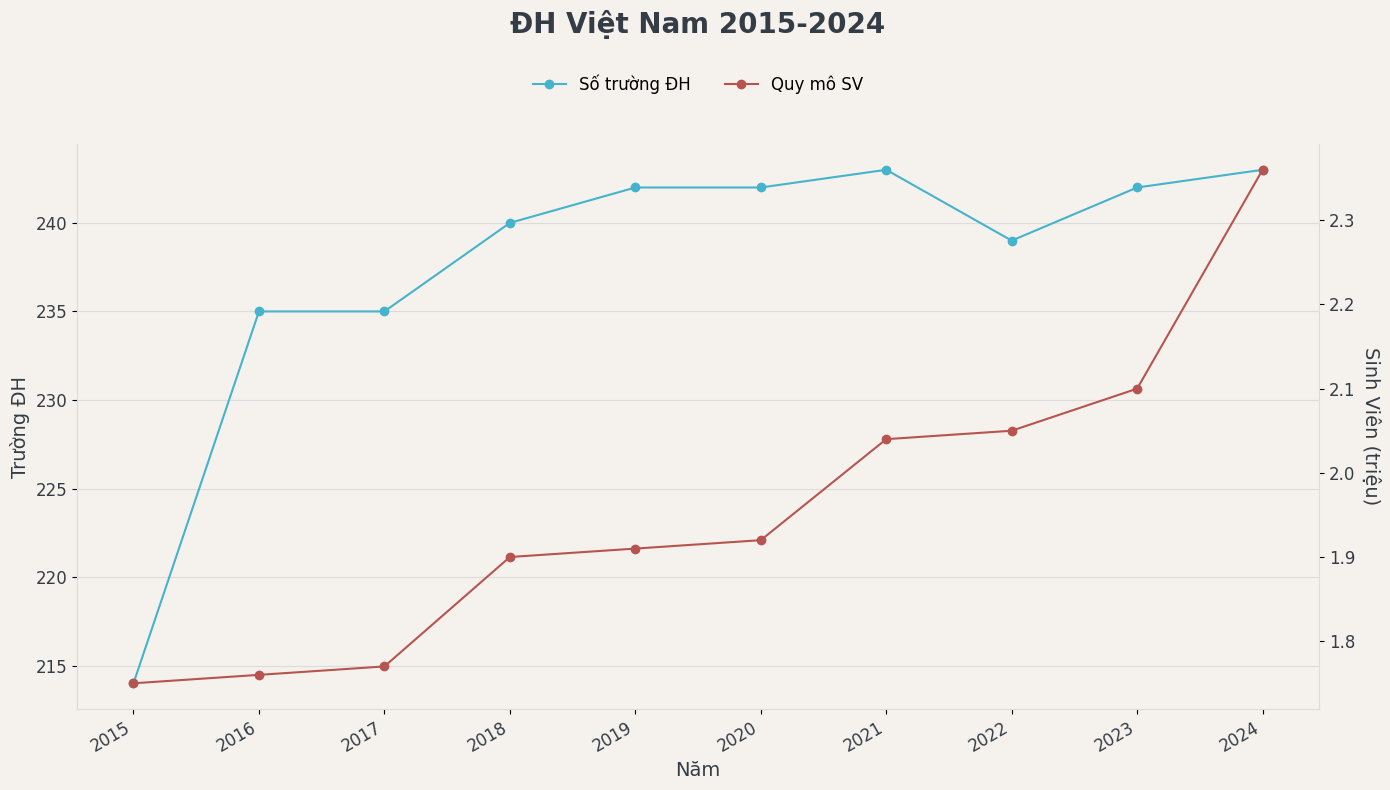
\includegraphics[width=\textwidth]{image/dh_viet_nam_2015_2024.png}
    \caption{越南高等教育办学机构数量与学生规模发展情况(2015-2024年)}
    \label{fig:so_truong_quy_mo_sv}
\end{figure}

分析图\ref{fig:so_truong_quy_mo_sv}显示了两种同步但速度不同的增长趋势。
\begin{itemize}
    \item \textbf{关于网络(蓝色线):} 高等教育机构数量呈现稳定而坚实的增长趋势,从2015年的215所增至2024年的243所。这一增长虽然不算突变,但反映了政府在拓展办学机构网络方面的一贯政策,包括成立新大学和升级专科学校,旨在为全国民众提供多样化的学习机会。
    \item \textbf{关于学生规模(红色线):} 与学校数量的平稳增长形成对比的是,学生规模呈现出异常强劲的爆炸性增长。在经历了2015年至2021年的相对稳定期后,学生规模在最后三年(2022-2024)内从约205万猛增至超过\textbf{235万学生}。这一飞跃不仅体现了高等教育日益增长的吸引力,也表明该体系正承受着为前所未有的大量学生提供培养需求的巨大压力。
\end{itemize}

这一增长正逐步使越南更接近到2030年实现\textbf{每万人口260名大学生}的国家战略目标\footcite{sggp_en_3million_2030}。此外,它还体现在重要的国际指标——高等教育毛入学率(GER)上。世界银行和联合国教科文组织的数据显示,越南的毛入学率已从2000年的仅10.3\%飙升至2018年的28.6\%,并于\textbf{2022年达到创纪录的42.22\%}\footcite{worldbank_humancapital_2022}。这是一项值得称道的成就,显示了教育大众化政策的成功。

\subsubsection{改善投入资源质量}
在扩大规模的同时,该体系的投入资源质量也取得了显著改善,显示了在提升内在能力方面的有目的的投资。
\begin{itemize}
    \item \textbf{师资队伍质量:} 拥有研究生学历(硕士或博士)的大学教师比例几乎翻了一番,从2007年的47\%增至\textbf{2020年达到85\%}\footcite{worldbank_p178112}。对提升师资队伍水平的投资是一个基础性因素,有望直接转化为教学和研究质量。
    \item \textbf{科学研究能力:} 提升教师水平的成就已产生具体影响。越南人均在国际权威期刊上可引用的科学文献数量,在十年间(2010-2020)\textbf{增长了三倍}\footcite{worldbank_improvingperformance_2020}。这表明该体系的研究能力取得了飞跃式进展,正逐步与国际科学界接轨。
\end{itemize}

上述数字和图表描绘了一幅关于悖论第一面的乐观画面:一个正在强劲发展、在网络、学生规模乃至投入资源质量等各方面都在扩张的高等教育体系。这些是不可否认的成就,为一个现代化和国际化的高等教育体系奠定了坚实的基础。然而,这幅画面只是一个更为复杂的悖论的一半。当我们将这些关于“量”的成就与关于产出质量和体系效率的指标进行对比时,一个充满挑战和警示的另一面故事开始显现。悖论的第二面将在下一部分深入分析。



% het goi 1


\subsection{悖论的第二面:质量的潜在危机与不匹配}
\label{subsec:ve_thu_hai_nghich_ly}

与规模和投入资源令人印象深刻的增长图景相反的是,关于产出质量和体系可持续性的 alarming signals。如果说悖论的第一面是一曲增长数字的交响乐,那么第二面则是一个残酷的现实,体现在培养规模与满足劳动力市场能力之间的分化。图\ref{fig:nghich_ly_quy_mo_chat_luong}清晰地将这一悖论可视化。

\begin{figure}[h!]
    \centering
    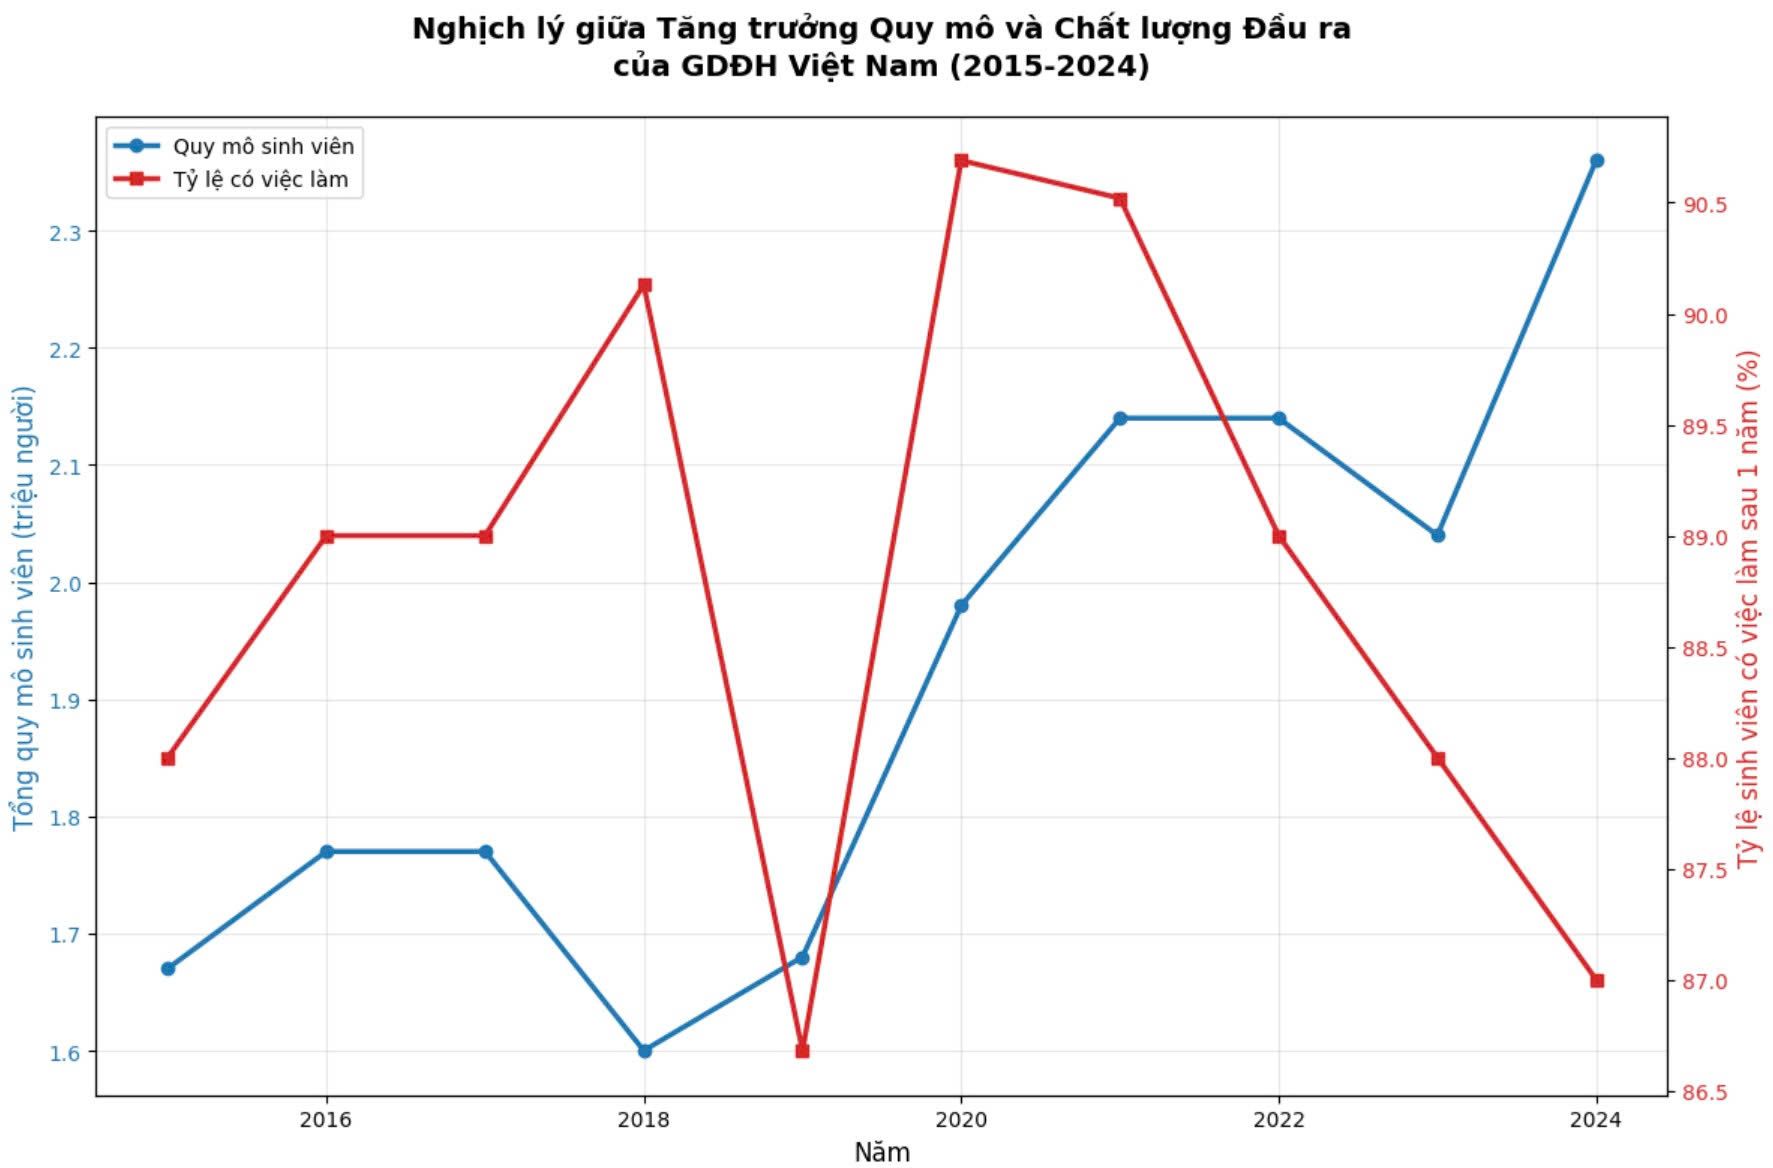
\includegraphics[width=\textwidth]{image/nghich_ly_tang_truong_quy_mo_chat_luong.jpg}
    \caption{越南高等教育规模增长与产出质量之间的悖论(2015-2024年)}
    \label{fig:nghich_ly_quy_mo_chat_luong}
    \vspace{0.2cm}
    \footnotesize{\textit{来源:综合整理自教育培训部数据及相关报告。}}
\end{figure}

\subsubsection{剖析“量”与“质”的分化}

图\ref{fig:nghich_ly_quy_mo_chat_luong}将两个重要指标置于同一坐标系中:学生总规模(左纵轴,蓝色线)和毕业一年后就业率(右纵轴,红色线)。理论上,在一个可持续发展的体系中,这两条线应呈正相关或至少保持稳定。然而,实际数据显示出一种令人担忧的分化(divergence):
\begin{itemize}
    \item \textbf{规模线(蓝色)}呈现出持续增长,特别是从2020年不到200万学生猛增至2024年超过230万学生。这再次证实了该体系面临的扩大规模的压力。
    \item \textbf{质量线(红色)}则呈现出完全相反的趋势。在2019-2020年左右达到峰值(超过90%)后,学生就业率出现了惊人的急剧下降,到2024年降至仅约87%。
\end{itemize}
这种分化正是发展悖论的“核心”:当体系在规模上日益“膨胀”时,其最核心的价值——帮助学习者获得就业并为社会做贡献的能力——却在下降。这提出了一个紧迫的问题:难道对数量的追求已经严重损害了质量?

\subsubsection{来自劳动力市场的证据:失业、技能差距与不平等}

图表中“质量”线的下降趋势并非感性判断,而是由一系列来自劳动力市场和社會學分析的確鑿數據所證實。

\paragraph{失业与学非所用。} 劳动荣军与社会部的报告多次警示本科毕业生失业率高企,\textbf{2017年高达23.7万人},2018年仍有\textbf{22.55万人},约占全国失业总人数的20\%\footcite{vietnamnews_unemployed_2017}。这一数字,加上估计约有\textbf{60\%的毕业生从事与专业不符的工作},是因培养与需求脱节而造成社会和个人资源浪费的明显证据\footcite{britishcouncil_grad_employability_2021}。

\paragraph{技能差距。} 上述状况的深层原因在于严重的“技能差距”。英国文化协会的一项全面调查指出了一个令人担忧的现实:\textbf{73\%}的越南企业在招聘具备领导和管理技能的人才时遇到困难;\textbf{68\%}在寻找具备足够专业技能的员工时遇到困难;\textbf{54\%}表示缺乏具备必要社交情感技能的人才\footcite{britishcouncil_skills_gap_2021}。世界银行的报告也强调,近\textbf{80\%}的制造业公司在招聘熟练工人时遇到困难\footcite{worldbank_p178112}。这表明培养方案并未能为学生充分装备经济真正需要的技能。

\paragraph{机会不均与财务负担。} 除了质量问题,发展悖论还体现在不平等方面。尽管越南高等教育的个人回报率位居世界最高之列(年均超过15\%)\footcite{worldbank_improvingperformance_2020},但这一利益并未得到公平分配。数据显示,高达\textbf{80\%来自收入最高20\%家庭的青年}已经或正在接受大学教育,而这一比例在两个最低收入组中仅占学生总数的10\%\footcite{worldbank_p178112}。由于成本负担日益转向家庭(占公立学校总收入的\textbf{77\%})以及学生贷款项目的缩减,这种不平等正面临着加剧的风险\footcite{worldbank_p178112}。

总之,悖论的第二面展示了一幅充满挑战的图景:一个尽管在规模和资源上投入巨大,但其产出却未能满足市场要求,同时潜藏着社会不平等风险的体系。清晰地认识这一悖论的两个方面,是能够准确“诊断”系统性“病症”的先决步骤,这一任务将在本章的后续部分进行。


% het goi 2



\section{塑造质量的主体与制度框架}
\label{sec:khung_the_che}

从已证明的“发展悖论”图景中,一个核心问题被提出:体系中的哪些力量和主体,以何种方式行动,从而造成了这一现状?要回答这个问题,首先需要识别主要的利益相关者,并分析主导该体系“游戏规则”的制度框架。

\subsection{高等教育质量保障生态系统中的利益相关者图}

越南高等教育质量保障体系是一个复杂的生态系统,有众多利益相关者参与其中,每一方都扮演着不同的角色、拥有不同的利益和影响力。图\ref{fig:so_do_he_thong_dbcl}提供了该生态系统中主要主体的概览。

\begin{figure}[h!]
    \centering
    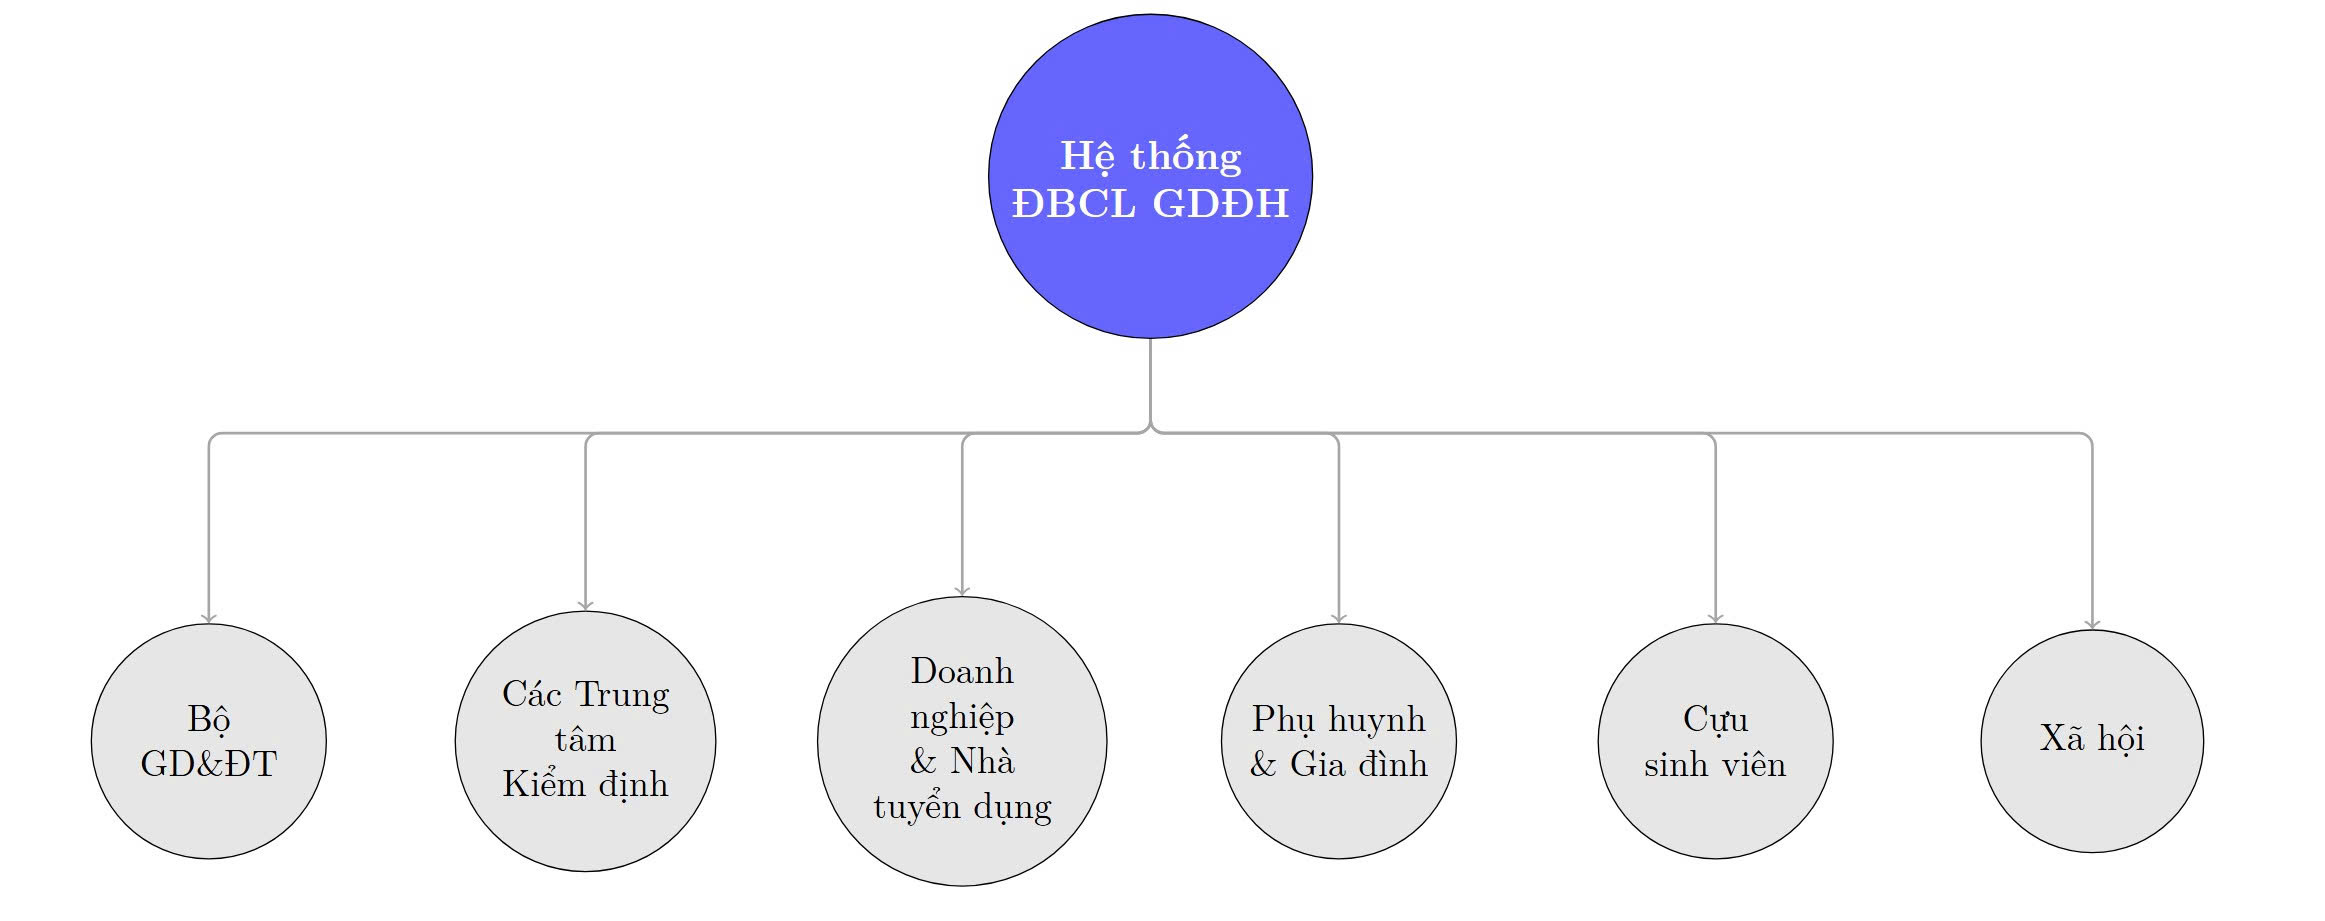
\includegraphics[width=\textwidth]{image/he_thong_dbcl_gddh.jpg}
    \caption{越南高等教育质量保障体系中的主要利益相关者图}
    \label{fig:so_do_he_thong_dbcl}
\end{figure}

上图可分为两大主要群体:
\begin{enumerate}
    \item \textbf{管理与执行群体(左侧与中心):} 包括国家机构和被直接授权的组织,扮演着制定政策和执行认证活动的角色。该群体包括\textbf{教育培训部}和各\textbf{认证中心}。
    \item \textbf{监督与受益群体(右侧):} 包括社会中的各个主体,他们是高等教育“产品”的直接使用者,并为质量提供重要的反馈。该群体包括\textbf{企业与雇主}、\textbf{家长与家庭}、\textbf{校友},以及更广泛的整个\textbf{社会}。
\end{enumerate}
分析这些主体,特别是制定“游戏规则”的群体之间的角色和关系,将阐明正在塑造越南质量保障现状的动因和压力。

\subsection{教育培训部:游戏规则的制定者与合规性压力}
\label{subsec:vai_tro_moet}

在越南的质量保障生态系统中,教育培训部扮演着核心权力主体的角色,负责构建和协调整个体系。从委托代理理论的视角来看,教育培训部是最高的“委托人”,将培养和保障质量的任务委托给各大学(代理人)\footcite{Kivisto2008}。同时,根据新制度主义理论,该部是产生最强大“强制性压力”的源头,迫使各大学遵守一个共同的法规框架,以获得合法性并维持运作\footcite{MeyerPowell2020}。

这种引领作用通过颁布一系列法规文件得以清晰体现,其核心精神由关于“根本性、全面性教育与培训革新”的第29号决议所指导\footcite{nghi_quyet_29_2013}。该决议明确提出了“增强教育培训机构的自主权和社会责任”以及建立一个“独立的认证体系”的要求。正是这些战略性导向,构建了法律走廊,推动各大学逐步与区域及国际标准接轨。

然而,这种集中的垂直管理机制,虽然对于确保统一性是必要的,但也正是导致许多教育机构形成一种\textbf{“合规文化”}而非\textbf{“改进文化”}的根本原因之一\footcite{pham2021governance}。各大学,特别是严重依赖国家预算的公立大学,倾向于优先开展旨在满足该部的报告要求和认证标准的活动,有时会轻视来自内部的实质性改进。因此,教育培训部既扮演着“游戏规则”制定者的角色,又是最高监督者,创造了一个合规性通常被置于创新之上的制度环境。

\subsection{质量认证中心:政策执行与独立性问题}
\label{subsec:vai_tro_trungtamkd}

如果说教育培训部是“委托人”,那么各教育质量认证中心则扮演着重要的“代理人”角色,其任务是具体化和执行认证政策。这些中心体系的发展,是越南质量保障活动制度化努力的证明。截至2024年初,全国共有7家获准运营的教育质量认证中心,包括公立和私立单位\footcite{tuoitre_kdcl_stats_2024}。

该体系已积极运作,在执行国家质量政策方面扮演着重要的“延伸手臂”角色。截至2023年底,这些中心已对全国\textbf{1855个培养项目}和\textbf{187所教育机构}进行了认证和承认\footcite{tuoitre_kdcl_stats_2024}。2021年两家私立中心的成立,也标志着朝着社会化、评估单位多样化方向迈出了新的一步。

然而,学术界和管理层提出的一个重要问题是这些中心的\textbf{实质性独立性}。尽管是以独立法人身份成立,但7家中心中有5家仍是大型大学或协会的下属单位,并且所有中心都在教育培训部的严密监督下运作。这种“既是主管单位,又是被认证对象”的关系,可能会引起人们对评估结果绝对客观性的怀疑\footcite{giaoducnet_kdcl_list_2023}。更重要的是,它有可能会进一步强化大学的合规压力。许多学校并未将认证中心视为共同改进的伙伴,而是仍然抱着应付上级“检查”的心态。这种复杂的关系将在后续章节中,在审视质量文化和体系协调等挑战时进行更深入的分析。


% het goi 3




























